%Centralizar verticalmente.
\newenvironment{midpage}{\vspace*{\fill}}{\vspace*{\fill}}
%Centralizar horizontalmente.
\newenvironment{midline}{\hspace*{\fill}}{\hspace*{\fill}}
\documentclass[12pts]{article}
\usepackage[utf8]{inputenc}
%Pacote para colocar cor no código.
\usepackage{color}
\definecolor{light-gray}{gray}{0.95}
%Pacote para inserir código.
\usepackage{listings}
\lstset{
    numbers=left,
    tabsize=2,
    backgroundcolor=\color{light-gray},
}
\title{
	Prática de Eletrônica Digital 1 - (119466)
	\singlespacing
		Turma E (Unb - Gama)
	\singlespacing
	\begin{midpage}
	\begin {large}
		Pré-Relatório Experimento 6
		\singlespace
		Introdução ao projeto em FPGA
	\end {large}
	\end{midpage}
}
\date{Outubro 04, 2016}
\usepackage{indentfirst}
\usepackage{setspace}
\usepackage{verbatim}
\usepackage[pdftex]{hyperref}
\usepackage{graphicx}
\begin{document}
\maketitle	
%\vspace{100 mm}
\begin{center}

\begin{tabular}{|c|l|r|}
\hline
Nome & Matrícula & Assinatura\\
\hline
Arthur Temporim & 140016759 & \\
\hline	
Eduardo Nunes & 140056149 & \\
\hline	
\end{tabular}

\end{center}

\pagebreak

\section{Pesquisa bibliográfica}

	Na seção a seguir contém as atividades pedidas para a elaboração do pré-relatório.
\singlespacing
\textit{\textbf{A)} As formas de alimentação suportadas pela placa, os níveis de tensão e corrente envolvidos e como esta configuração é feita:}


\textbf{ Formas de alimentação:} A placa Basys3 pode receber energia da porta Digilent USB-JTAG(J4) ou a partir de uma fonte de alimentação externa 5V.
\singlespacing
\textbf{Níveis de tensão:} É necessário limitar a tensão máxima da bateria externa a 5.5V DC. A tensão mínima da bateria depende da aplicação; se a função de host USB (J2) estiver sendo utilizada, pelo menos,
4.6V deve ser fornecida. Em outros casos, a voltagem mínima é de 3.6V.
\singlespacing
\textbf{Corrente envolvidas:} É necessário 3.3, 1.8V e suprimentos de 1.0V a partir da entrada 5V de alimentação principal.
\singlespacing
\textbf{Para configurar o FPGA, há três maneiras:}
\singlespacing
1. O PC pode usar o circuito Digilent USB-JTAG (portJ4, identificado como "PROG") para programar o FPGA para que a qualquer momento o aparelho esteja ligado.
\singlespacing
2. Um ficheiro armazenado no de série (SPI) dispositivo flash não volátil pode ser transferido para o FPGA usando a porta SPI.
\singlespacing
3. Um arquivo de programação podem ser transferidos a partir de um cartão de memória USB ligado ao HID USB port.
\singlespacing
\textit{\textbf{B)} As formas de programação suportadas pela placa e como elas podem ser configuradas:}
        Você pode programar o FPGA a partir de um pen drive conectado à porta USB-HID (J2). Ou através da programação JTAG pode ser feito usando o servidor de hardware em Vivado. Ou com um circuito que pode programar dispositivos flash.
\singlespacing
\textit{\textbf{C)} As formas de armazenamento do bitstream na placa (tipos de memória):}
        A placa Basys3 contém um dispositivo serial flash 32Mbit não-volátil, que está ligado ao FPGA Artix 7 usando um quad-modo dedicado (x4) barramento SPI.
\singlespacing
\textit{\textbf{D}) A quantidade e frequência dos clocks disponíveis:}
A placa Basys3 inclui um único oscilador de 100MHz conectada ao pino W5 (W5 é uma entrada no banco de MRCC 34).
\singlespacing
\textit{\textbf{E)} A identificação (nome) dos pinos usados para as entradas da placa (chaves e pushbuttons) e para as saídas (LEDs e displays de 7-segmentos):}
\begin{figure}[!htb]
  \centering
  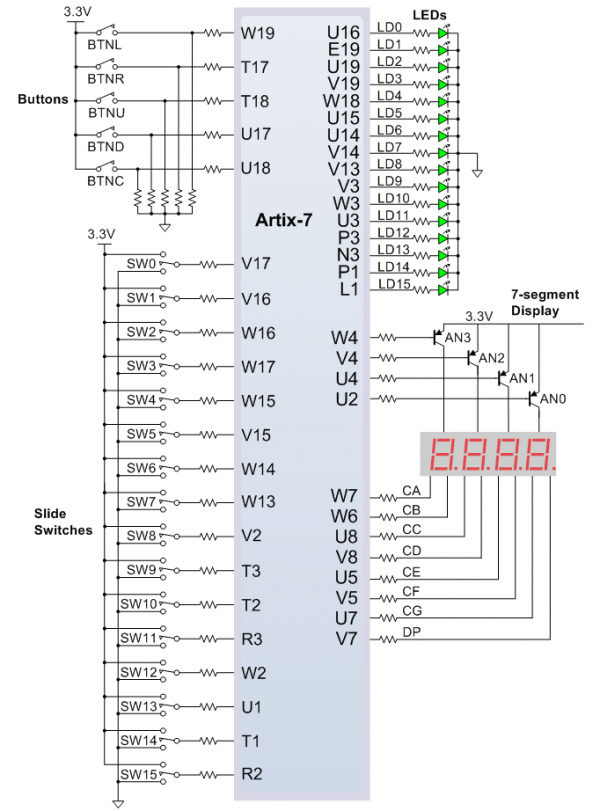
\includegraphics[scale=0.3]{imagens/identificacaoPinos.png}
  \caption{Identificação dos pinos - Ise Design Suit 14.7}
  \label{figRotulo}
\end{figure}


\section{Projetos e simulações}

\subsection{Projeto 1}

Este circuito consiste na simples exibição em LEDs de acordo com os valores de entrada nos \textit{switchs} de uma placa FPGA.

\subsubsection{Diagrama Esquemático}

\begin{figure}[!htb]
  \centering
  
\includegraphics[scale=0.3	]{imagens/esquematico1}
  \caption{Diagrama 1 - Ise Design Suit 14.7}
  \label{figRotulo}
\end{figure}

\subsubsection{Código VHDL}
%\lstinputlisting[language=vhdl]{projetos/projeto1/projeto1.vhd}

\pagebreak

\subsection{Projeto 2}

Este circuito consiste em mostra os valores de 2 números de 4 bits cada em 2 displays de BCD utilizando multiplexadores e clocks para representar o resultado.

\subsubsection{Código VHDL}
\lstinputlisting[language=vhdl]{projetos/projeto2/projeto2.vhd}
\end{document}